\documentclass[
11pt, % Set the default font size, options include: 8pt, 9pt, 10pt, 11pt, 12pt, 14pt, 17pt, 20pt
%t, % Uncomment to vertically align all slide content to the top of the slide, rather than the default centered
%aspectratio=169, % Uncomment to set the aspect ratio to a 16:9 ratio which matches the aspect ratio of 1080p and 4K screens and projectors
]{beamer}

\graphicspath{{images/}{./}} % Specifies where to look for included images (trailing slash required)

\usepackage{watermark}
\usepackage{graphicx}  % Para incluir imágenes si deseas usar una imagen como marca de agua
\usepackage{array}
\usepackage[utf8]{inputenc}
\usepackage[spanish]{babel}
\usepackage{circuitikz} % Paquete para diagramas de circuitos eléctricos
\usepackage{tikz}
\usetikzlibrary{shapes.geometric, arrows.meta, positioning}
\usepackage{smartdiagram}
\usepackage{eso-pic}

\usepackage{booktabs}
\usepackage[table,xcdraw]{xcolor}


% Agregar logo
\logo{
\includegraphics[width=1cm]{logo.jpeg}} % Cambia "logo.png" por la ruta de tu imagen

\usepackage{booktabs} % Allows the use of \toprule, \midrule and \bottomrule for better rules in tables

%----------------------------------------------------------------------------------------
%	SELECT LAYOUT THEME
%----------------------------------------------------------------------------------------

% Beamer comes with a number of default layout themes which change the colors and layouts of slides. Below is a list of all themes available, uncomment each in turn to see what they look like.

%\usetheme{default}
%\usetheme{AnnArbor}
%\usetheme{Antibes}
%\usetheme{Bergen}
%\usetheme{Berkeley}
%\usetheme{Berlin}
%\usetheme{Boadilla}
%\usetheme{CambridgeUS}
%\usetheme{Copenhagen}
%\usetheme{Darmstadt}
%\usetheme{Dresden}
%\usetheme{Frankfurt}
%\usetheme{Goettingen}
%\usetheme{Hannover}
%\usetheme{Ilmenau}
%\usetheme{JuanLesPins}
%\usetheme{Luebeck}
\usetheme{Madrid}
%\usetheme{Malmoe}
%\usetheme{Marburg}
%\usetheme{Montpellier}
%\usetheme{PaloAlto}
%\usetheme{Pittsburgh}
%\usetheme{Rochester}
%\usetheme{Singapore}
%\usetheme{Szeged}
%\usetheme{Warsaw}

%----------------------------------------------------------------------------------------
%	SELECT COLOR THEME
%----------------------------------------------------------------------------------------

% Beamer comes with a number of color themes that can be applied to any layout theme to change its colors. Uncomment each of these in turn to see how they change the colors of your selected layout theme.

%\usecolortheme{albatross}
%\usecolortheme{beaver}
%\usecolortheme{beetle}
%\usecolortheme{crane}
%\usecolortheme{dolphin}
%\usecolortheme{dove}
%\usecolortheme{fly}
%\usecolortheme{lily}
%\usecolortheme{monarca}
%\usecolortheme{seagull}
%\usecolortheme{seahorse}
%\usecolortheme{spruce}
%\usecolortheme{whale}
%\usecolortheme{wolverine}

%----------------------------------------------------------------------------------------
%	SELECT FONT THEME & FONTS
%----------------------------------------------------------------------------------------

% Beamer comes with several font themes to easily change the fonts used in various parts of the presentation. Review the comments beside each one to decide if you would like to use it. Note that additional options can be specified for several of these font themes, consult the beamer documentation for more information.

\usefonttheme{default} % Typeset using the default sans serif font
%\usefonttheme{serif} % Typeset using the default serif font (make sure a sans font isn't being set as the default font if you use this option!)
%\usefonttheme{structurebold} % Typeset important structure text (titles, headlines, footlines, sidebar, etc) in bold
%\usefonttheme{structureitalicserif} % Typeset important structure text (titles, headlines, footlines, sidebar, etc) in italic serif
%\usefonttheme{structuresmallcapsserif} % Typeset important structure text (titles, headlines, footlines, sidebar, etc) in small caps serif

%------------------------------------------------

%\usepackage{mathptmx} % Use the Times font for serif text
\usepackage{palatino} % Use the Palatino font for serif text

%\usepackage{helvet} % Use the Helvetica font for sans serif text
\usepackage[default]{opensans} % Use the Open Sans font for sans serif text
%\usepackage[default]{FiraSans} % Use the Fira Sans font for sans serif text
%\usepackage[default]{lato} % Use the Lato font for sans serif text

%----------------------------------------------------------------------------------------
%	SELECT INNER THEME
%----------------------------------------------------------------------------------------

% Inner themes change the styling of internal slide elements, for example: bullet points, blocks, bibliography entries, title pages, theorems, etc. Uncomment each theme in turn to see what changes it makes to your presentation.

%\useinnertheme{default}
\useinnertheme{circles}
%\useinnertheme{rectangles}
%\useinnertheme{rounded}
%\useinnertheme{inmargin}

%----------------------------------------------------------------------------------------
%	SELECT OUTER THEME
%----------------------------------------------------------------------------------------

% Outer themes change the overall layout of slides, such as: header and footer lines, sidebars and slide titles. Uncomment each theme in turn to see what changes it makes to your presentation.

%\useoutertheme{default}
%\useoutertheme{infolines}
%\useoutertheme{miniframes}
%\useoutertheme{smoothbars}
%\useoutertheme{sidebar}
%\useoutertheme{split}
%\useoutertheme{shadow}
%\useoutertheme{tree}
%\useoutertheme{smoothtree}

%\setbeamertemplate{footline} % Uncomment this line to remove the footer line in all slides
%\setbeamertemplate{footline}[page number] % Uncomment this line to replace the footer line in all slides with a simple slide count

%\setbeamertemplate{navigation symbols}{} % Uncomment this line to remove the navigation symbols from the bottom of all slides

%----------------------------------------------------------------------------------------
%	PRESENTATION INFORMATION
%----------------------------------------------------------------------------------------

\title[Metodología de Investigación]{Metodología para el estudio universitario} % The short title in the optional parameter appears at the bottom of every slide, the full title in the main parameter is only on the title page

%\subtitle{Optional Subtitle} % Presentation subtitle, remove this command if a subtitle isn't required

\author[Edison Achalma]{Edison Achalma} % Presenter name(s), the optional parameter can contain a shortened version to appear on the bottom of every slide, while the main parameter will appear on the title slide

\institute[CAU - UNSCH]{Corporación Académica Universitaria CAU - UNSCH \\ \smallskip \textit{achalmed.18@gmail.com}} % Your institution, the optional parameter can be used for the institution shorthand and will appear on the bottom of every slide after author names, while the required parameter is used on the title slide and can include your email address or additional information on separate lines

\date[\today]{Sesión 03 actualizado \\ \today} % Presentation date or conference/meeting name, the optional parameter can contain a shortened version to appear on the bottom of every slide, while the required parameter value is output to the title slide

%----------------------------------------------------------------------------------------


\begin{document}
% Página de título
\begin{frame}
	\titlepage
\end{frame}

% Diapositiva de contenido
% Configuración: Incluir índice automáticamente en cada sección

\AtBeginSection[]{
	\begin{frame}{Índice de la Sección}
		\tableofcontents[currentsection] % Índice automático de la sección actual
	\end{frame}
}



% Sección 7
\section{Citas}
\begin{frame}
	\frametitle{Citas en APA}
	\begin{block}{}
		\textbf{Cita:} Cada vez que utilices ideas de otros autores, deberás dar crédito a estas ideas. El acto de creditar estas palabras es conocido como \textbf{Citas}.
	\end{block}

	Entonces “Citar algo” significa dar crédito a ideas, frases o pensamientos de otros. No citar adecuadamente puede llevar a acusaciones de plagio, con repercusiones académicas y legales.

	\textbf{Sistema de Citación APA:}

	El estilo APA usa el formato \textbf{Autor-Fecha} para las citas, donde se menciona el apellido del autor y el año de la publicación.

	\begin{alertblock}{Importante:}
		Todas las fuentes citadas en el texto deben aparecer en la lista de referencias al concluir tu trabajo.
	\end{alertblock}
\end{frame}


\begin{frame}
	\frametitle{Estructura de las Citas}

	\textbf{Elementos clave:}
	\begin{itemize}
		\item Autor(es).
		\item Año de publicación.
		\item Número de página (solo en citas textuales).
	\end{itemize}

	\textbf{Formatos básicos:}

		\begin{columns}[T] % Alineación superior de las columnas
		\column{0.5\textwidth}
		\begin{block}{Cita narrativa}
			\begin{itemize}
				\item El autor se incluye en la redacción del párrafo. La fecha se pone entre paréntesis. \item Énfasis en el autor.
				\item Implica el uso de frases de citación.
			\end{itemize}
		\end{block}
		\vspace{0.1cm}
		\column{0.5\textwidth}
		\begin{block}{Cita parentética}
			\begin{itemize}
				\item Se menciona la idea y los datos de autor y fecha aparecen entre paréntesis.
				\item Énfasis en el texto.
				\item No implica el uso de frases de citación.
			\end{itemize}
		\end{block}
	\end{columns}

\end{frame}

\begin{frame}
	\frametitle{Citas narrativas}
	\textbf{Cita narrativa (basada en el autor):} Aquí, el nombre del autor se incorpora como parte de la oración y el año entre paréntesis.

	\begin{exampleblock}{}
\begin{figure}
	\centering
	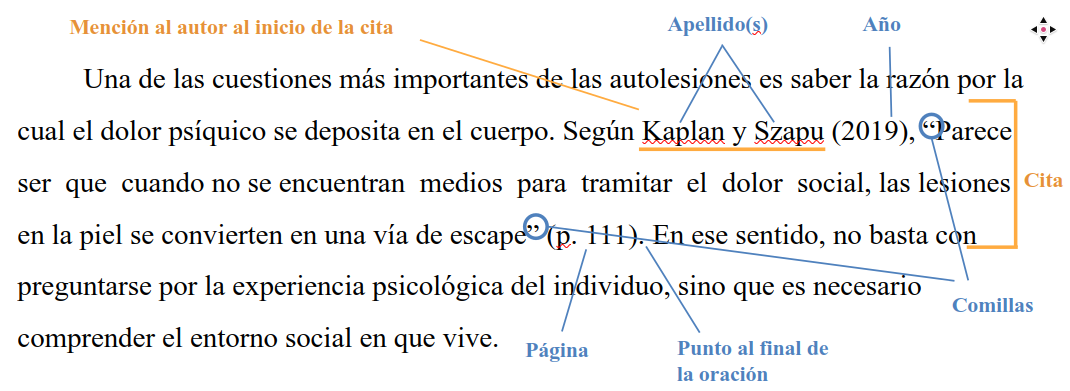
\includegraphics[width=1\linewidth]{images/screenshot001}
	\caption{Cita narrativa}
	\label{fig:screenshot001}
\end{figure}

	\end{exampleblock}

\end{frame}

\begin{frame}
	\frametitle{Citas en paréntesis}

	\textbf{Cita en paréntesis/parentética (basada en el texto):} El nombre del autor y la fecha aparecen entre paréntesis al final de la cita.

	\begin{exampleblock}{}
		\begin{figure}
			\centering
			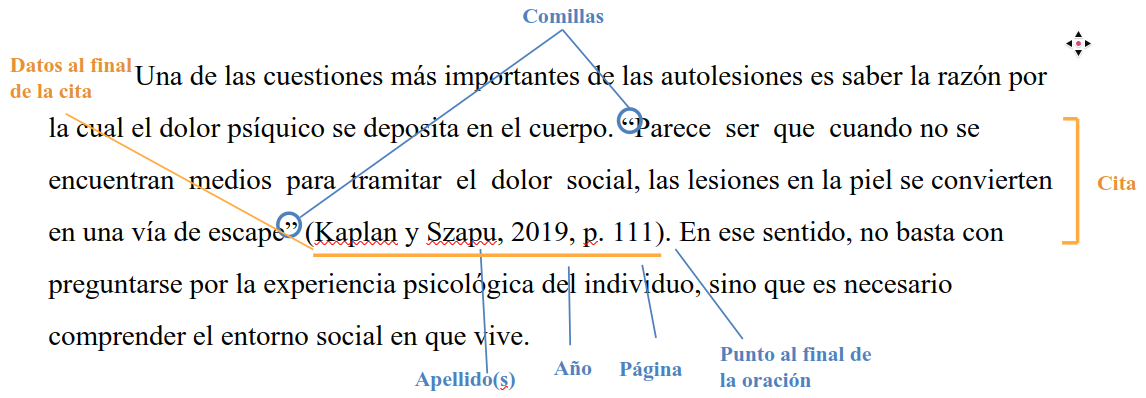
\includegraphics[width=1\linewidth]{images/screenshot002}
			\caption{Cita en paréntesis}
			\label{fig:screenshot002}
		\end{figure}

	\end{exampleblock}

\end{frame}


\begin{frame}
	\frametitle{Citando Corporaciones, Instituciones o Fundaciones}
	\begin{itemize}
		\item Puede citar a entidades como autor en lugar de individuos.
		\item Use abreviaturas solo si son ampliamente conocidas (ej.: ONU).
		\item Para entidades menos conocidas, use el nombre completo en la primera cita, seguido de la abreviatura entre corchetes, y luego solo la abreviatura en citas subsiguientes.
	\end{itemize}

	\begin{exampleblock}{Ejemplo cita en paréntesis}
		\begin{itemize}
			\item \textbf{Primera cita en el texto:} \\(Asociación Americana para el Avance de la Ciencia {\color{blue}[}AAAC{\color{blue}]}, 2014, p. 18)
			\item \textbf{Siguientes citas:} \\ (AAAC, 2014, p. 90)
		\end{itemize}.
	\end{exampleblock}
\end{frame}

\begin{frame}
	\frametitle{Citando Corporaciones, Instituciones o Fundaciones}
	\begin{exampleblock}{Ejemplo cita narrativa}
		\begin{itemize}
			\item \textbf{Primera cita en el texto:} \\Asociación Americana para el Avance de la Ciencia (AAAC, 2014)
			\item \textbf{Siguientes citas:} \\ AAAC (2014)
		\end{itemize}.
	\end{exampleblock}

	\textbf{Recomendaciones:}

	\begin{itemize}
		\item \textbf{Verificación de Citas:} Todo autor en las referencias debe haber sido citado en el texto, ya sea textual o parafraseado.
	\end{itemize}

	\begin{itemize}
		\item \textbf{Citas de Fuentes Primarias:} Prefiera citar fuentes primarias. {\color{blue}Si una fuente (Libro A) cita otra (Libro B), busque el Libro B para citarlo directamente.}
	\end{itemize}

	\begin{itemize}
		\item Evite la subcitación (pocas citas) para prevenir plagio o auto-plagio y la sobrecitación (muchas citas), que puede distraer al lector.
	\end{itemize}
\end{frame}


\begin{frame}
	\frametitle{Tipos de Citas en APA}

	El estilo APA distingue entre dos principales tipos de citas:

	\textbf{Citas Textuales:}

	Se refieren a cuando reproduces exactamente las palabras de un autor.
	\begin{block}{Menos de 40 palabras:}
		Se integran en el texto con comillas dobles y se cita el autor, año y número de página.
	\end{block}
	\begin{block}{Más de 40 palabras:}
		Se presentan en un bloque, sangradas 0.5 pulgadas (1.27cm) del margen izquierdo, sin comillas.
	\end{block}

	\textbf{Citas Parafraseadas:}

	Son aquellas donde expresas en tus propias palabras las ideas de otro autor.

\end{frame}


% Sección
\subsection{Cita textual o Directa}

\begin{frame}
	\frametitle{Cita textual o directa}

	\begin{block}{}
		Una cita es textual o directa cuando se reproduce palabra por palabra de un texto de otro autor o incluso de su propio texto ya escrito en otra publicación. Debes informar:
	\end{block}

	\begin{itemize}
		\item Autor y año.
		\item Página específica (o detalles para casos sin paginación).
		\item Referencia completa en la lista de referencias.
	\end{itemize}

	\textbf{Sugerencias:}
	\begin{itemize}
		\item Preferir el parafraseo para ajustar el material al contexto de tu trabajo de investigación.
		\item Usar citas textuales para:
		      \begin{itemize}
			      \item {\color{blue}Frases memorables o sucintas.}
			      \item {\color{blue}Reproducir definiciones exactas.}
		      \end{itemize}
	\end{itemize}
	\textbf{Nota:} Ten en cuenta que algunos profesores pueden establecer límites en el uso de citas directas.
\end{frame}

\begin{frame}
	\frametitle{Ejemplo de cita textual corta}

	Para citas de menos de 40 palabras:

	\begin{exampleblock}{Cita narrativa (énfasis en el autor)}
		Analizando la crisis financiera del 2008, {\color{blue}Lynch (2012)} afirma que {\color{blue}``}la crisis ha sido motivada por lo que hay de más perverso en el mundo capitalista{\color{blue}'' (p. 127)}, contribuyendo a un clima general de negatividad con los partidos de derecha.
	\end{exampleblock}

	\begin{exampleblock}{Cita entre paréntesis (énfasis en la cita)}
		Varios economistas han afirmado en la crisis financiera del 2008 que {\color{blue}``}la crisis ha sido motivada por lo que hay de más perverso en el mundo capitalista{\color{blue}'' (Lynch, 2012, p. 127)} lo que ha contribuido para un malestar con los partidos de derecha por el mundo.
	\end{exampleblock}

\end{frame}

\begin{frame}
	\frametitle{Ejemplo de cita textual larga}

	\begin{exampleblock}{}
		\begin{figure}
			\centering
			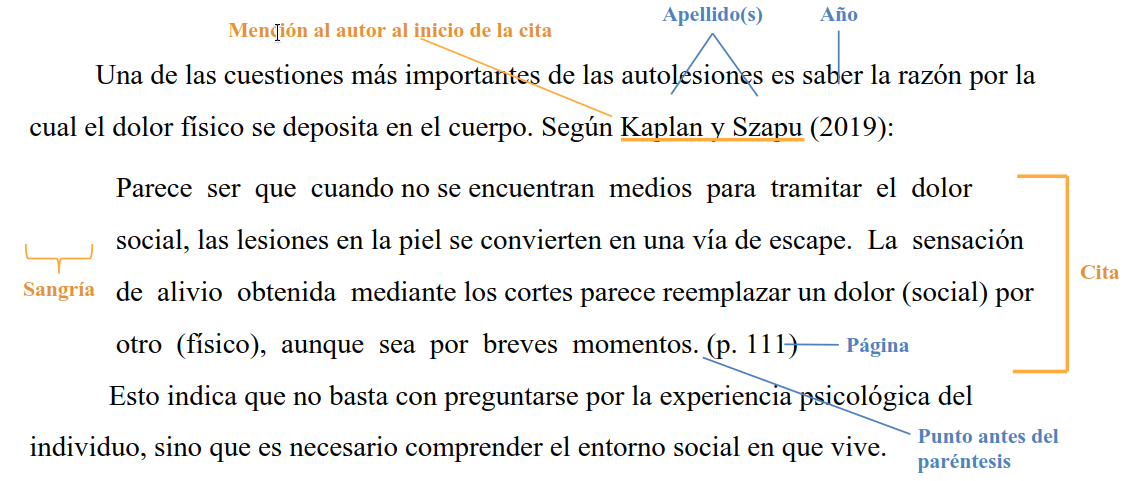
\includegraphics[width=1\linewidth]{images/screenshot003}
			\caption{Cita narrativa}
			\label{fig:screenshot003}
		\end{figure}
	\end{exampleblock}

\end{frame}

\begin{frame}
	\frametitle{Ejemplo de cita textual larga}

	\begin{exampleblock}{}
		\begin{figure}
			\centering
			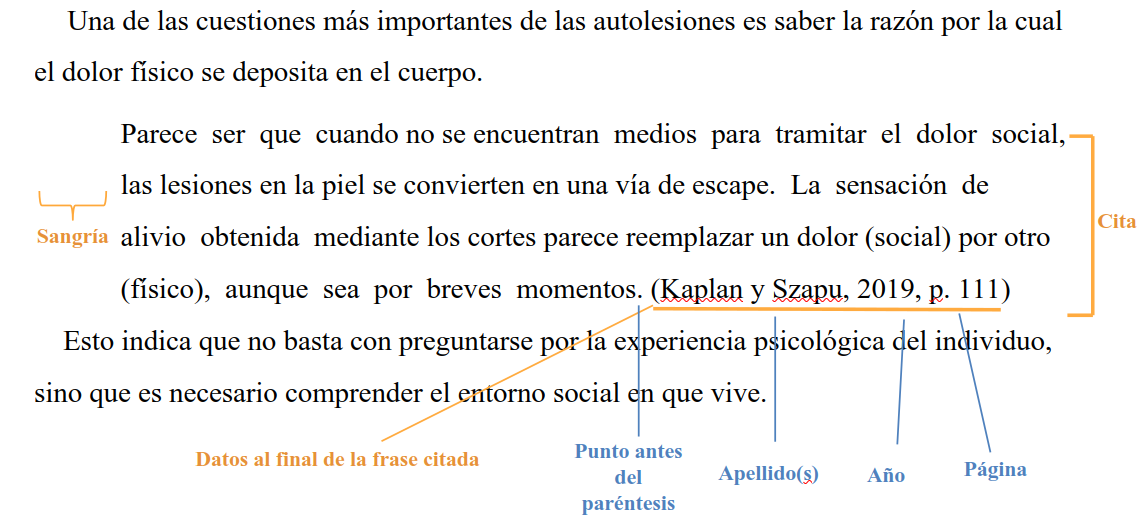
\includegraphics[width=1\linewidth]{images/screenshot004}
			\caption{Cita en paréntesis}
			\label{fig:screenshot004}
		\end{figure}
	\end{exampleblock}

\end{frame}

\begin{frame}
	\frametitle{Citas con errores}

	Evite citar con errores gramaticales u ortográficos. Si es necesario:
	\begin{itemize}
		\item Mantenga la cita como en la fuente original.
		\item Inserte la palabra ``\textit{[sic]}'', en cursiva y entre corchetes, inmediatamente después del error en la cita.
	\end{itemize}

	\begin{exampleblock}{Ejemplo}
		Martinello (2017) escribió que ``el {\color{red}serumano} \textit{{\color{blue}[sic]}} es la peor plaga que ha aparecido en la tierra'' (p. 24).
	\end{exampleblock}

	\textbf{Nota:} Una buena solución es parafrasear en vez de citar textualmente.

\end{frame}

\begin{frame}
	\frametitle{Modificaciones en las citas}

	\textbf{Cambios sin explicación:}
	\begin{itemize}
		\item Mayúsculas o minúsculas al inicio de la cita.
		\item Algunos signos de puntuación al final, {\color{red}siempre que no se cambie el significado}.
		\item Comillas simples a dobles y viceversa.
		\item Omitir notas al pie del original.
	\end{itemize}

	\textbf{Cambios en una cita que requieren explicación:}
	\begin{itemize}
		\item Puntos suspensivos para \textbf{omisiones} de palabras dentro de una cita.
		\item Tres puntos (. . .) o carácter de puntos suspensivos (…).
		\item Cuatro puntos (. …) para salto de oraciones.
		\item Corchetes [ ] para adiciones o explicaciones.
		\item Cursiva para énfasis con "[cursivas añadidas]".
	\end{itemize}

	\begin{exampleblock}{Ejemplo}
		Según Sánchez (2020), ``más raro que no haber encontrado vida {\color{blue}[extraterrestre]}, es que ellos todavía {\color{blue}…} no han podido encontrarnos'' (p. 40).
	\end{exampleblock}

\end{frame}

\begin{frame}
	\frametitle{Materiales con paginación}

	\textbf{Al citar directamente, siempre proporcione el autor, el año y el número de página de la cita} (tanto en citas entre paréntesis como narrativas en el texto).

	Siga estas pautas cuando proporcione un número de página:
	\begin{itemize}
		\item Para una sola página, use la abreviatura “p.” (ejemplo: \textbf{p. 25}).
		\item Para varias páginas, use la abreviatura “pp.” Y separe el rango de página con un guión en (ejemplo: \textbf{pp. 34–36}).
		\item Si las páginas son discontinuas, use una coma entre los números de página (ejemplo: \textbf{págs. 67, 72}).
		\item Si el trabajo no tiene números de página, proporcione otra forma para que el lector localice la cita (ejemplo: \textbf{cap. 5, párr. 4}).
	\end{itemize}

\end{frame}

\begin{frame}
	\frametitle{Omitiendo algunas palabras de una cita textual}

	Cuando queremos omitir parte del material original podemos utilizar los puntos suspensivos. \textbf{Estos deben ser representados por tres puntos separados por espacio.}

	\begin{itemize}
		\item \textbf{Al final o comienzo:} Generalmente innecesario, a menos que se requiera aclarar.
		\item \textbf{En el medio de una oración:} Para omitir material no pertinente.
		\item \textbf{Para múltiples oraciones:} Cuatro puntos (. . . .) para indicar omisión entre oraciones.
	\end{itemize}

	\begin{exampleblock}{Puntos suspensivos al final o comienzo de una cita}
		En la visión de Nietzsche (1878) ``{\color{blue}. . .} es una cultura de hombres. Por lo que a las mujeres respecta, todo lo dice Pericles en el discurso fúnebre con las palabras: tanto mejores son cuanto entre los hombres se habla de ellas lo menos posible.''
	\end{exampleblock}

\end{frame}

\begin{frame}
	\frametitle{Omitiendo algunas palabras de una cita textual}

	\begin{exampleblock}{Puntos suspensivos en el medio una oración}
		De acuerdo a Nietzsche (1878) ``la cultura griega del periodo clásico es una cultura de hombres. Por lo que a las mujeres respecta, todo lo dice Pericles en el discurso fúnebre con las palabras: tanto mejores son cuanto entre los hombres se habla de ellas lo menos posible. La relación erótica de los hombres con los adolescentes{\color{blue} . . .} todo el idealismo de la fuerza de la naturaleza griega se vertió en esa relación''
	\end{exampleblock}

	\begin{exampleblock}{Puntos suspensivos para omitir múltiples oraciones}
		Según Nietzsche (1878) ``la cultura griega del periodo clásico es una cultura de hombres{\color{red}.} {\color{blue}. . .} todo el idealismo de la fuerza de la naturaleza griega se vertió en esa relación y probablemente jamás han vuelto nunca los jóvenes a ser tratados tan atenta, tan amorosamente''
	\end{exampleblock}

\end{frame}



% Sección
\subsection{Cita parafraseadas}

\begin{frame}
	\frametitle{¿Qué es una cita de parafraseo?}

	\begin{block}{}
		En la cita de parafraseo, se utilizan las ideas de un autor pero expresadas en palabras propias del escritor. La paráfrasis reafirma la idea de otro autor en tus propias palabras, permitiendo:
	\end{block}

	\begin{itemize}
		\item Resumir y sintetizar información.
		\item Enfocarse en lo significativo.
		\item Comparar y contrastar detalles.
	\end{itemize}

	\textbf{Siempre debes incluir:}
	\begin{itemize}
		\item Apellido del autor.
		\item Año de publicación.
		\item  Número de página: Es recomendable, pero no obligatorio.
	\end{itemize}

	\begin{alertblock}{Importante}
		Es aconsejable que, como autor, ejercite la práctica de parafrasear
	\end{alertblock}

\end{frame}

\begin{frame}
	\frametitle{Ejemplo de parafraseo narrativo}

	\begin{exampleblock}{}
		\begin{figure}
			\centering
			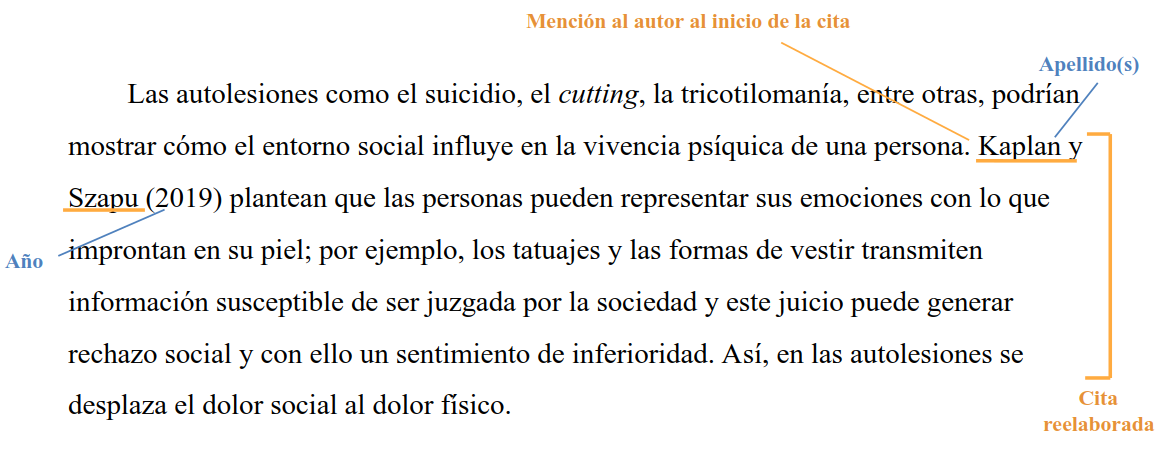
\includegraphics[width=1\linewidth]{images/screenshot005}
			\caption{Parafraseo narrativo}
			\label{fig:screenshot005}
		\end{figure}
	\end{exampleblock}
\end{frame}

\begin{frame}
	\frametitle{Ejemplo de parafraseo parentético}

	\begin{exampleblock}{}
		\begin{figure}
			\centering
			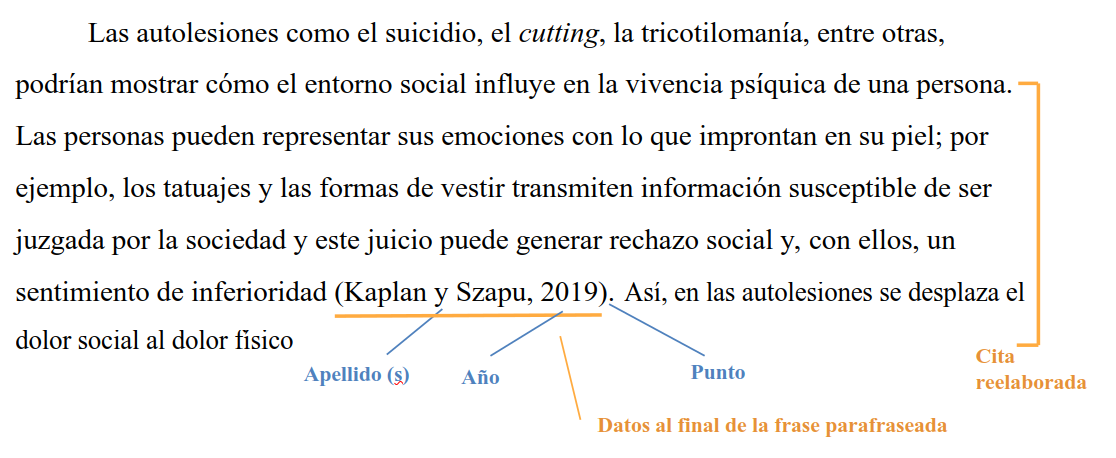
\includegraphics[width=1\linewidth]{images/screenshot006}
			\caption{parafraseo parentético}
			\label{fig:screenshot006}
		\end{figure}
	\end{exampleblock}
\end{frame}

\begin{frame}
	\frametitle{Una paráfrasis larga}

	Para paráfrasis de varias oraciones:

	\begin{itemize}
		\item Cite el trabajo en la primera mención.
		\item No es necesario repetir la cita si el contexto indica que se sigue parafraseando el mismo trabajo.
	\end{itemize}

	\begin{exampleblock}{Ejemplo}
		Según {\color{blue}Taleb (2019)} el crac bancario del 2018 fue por cuenta de una acumulación de riesgos ocultos y asimétricos y que los banqueros estaban empeñados en búsqueda de rentas. {\color{blue} Además, encontró} que la elección de Donald Trump era obvia ya, dijera lo que dijera, se presentaba al público como una persona verdadera, al contrario, de los otros candidatos.
	\end{exampleblock}

	\textbf{Nota:} Si la paráfrasis continúa en un nuevo párrafo, reintroduce la cita.

\end{frame}

\begin{frame}
	\frametitle{Más de una obra en la misma paráfrasis}

	Cuando la paráfrasis incluye múltiples fuentes:

	\begin{itemize}
		\item Repita la cita para mantener clara la fuente.
	\end{itemize}

	\begin{exampleblock}{Ejemplo}
		Varios economistas han encontrado que entre los motivos del crac del 2008 estuvo el exceso de apalancamiento de los bancos {\color{blue}(Taleb, 2019)}, el crédito subprime {\color{blue}(Sánchez et al., 2020)} y que estos dos factores han llevado a la formación de una burbuja inmobiliaria durante décadas {\color{blue}(Ayala y Masiero, 2010; Taleb, 2019)}. Todos estos factores han causado la peor caída de la bolsa americana en los últimos 50 años y más de diez bancos tuvieron que ser rescatados por el banco central americano {\color{blue}(Tabárez y Ferreira, 2010; Floyd et al., 2020; Oliveira, 2019)}.
	\end{exampleblock}

	\textbf{Importante:} Revise sus oraciones para asegurar que las fuentes están citadas correctamente.

\end{frame}



% Sección
\subsection{Cita con más de un autor}

\begin{frame}
	\frametitle{Citas con más de un autor}

	\textbf{Citas con dos autores}

	Siempre mencione ambos autores, sus apellidos van separados por “y” tanto en las citas narrativas como parentéticas. Esta es una propuesta de adaptación al español:

	\begin{exampleblock}{}
		(Suárez y Rodríguez, 2019)
	\end{exampleblock}

	\textbf{Citas de tres o más autores}

	Para tres o más autores, siempre use ``et al." (que significa “y otros”) después del primer autor:

	\begin{exampleblock}{Para Sánchez, Ferreira, Hermosillo, Minyang y Velling (2018)}
		\begin{itemize}
			\item \textbf{Primera vez en el texto:} Sánchez {\color{blue}et al.} (2018) afirman que la diversidad de género…
			\item … una perspectiva igualitaria entre los géneros (Morrison et al., 2015).
		\end{itemize}
	\end{exampleblock}

	\textbf{Nota:} Esta regla solo se aplica a citas, no a referencias bibliográficas.

\end{frame}



\begin{frame}
	\frametitle{Evitando ambigüedad en las citas}

	Para evitar confusiones cuando hay múltiples obras con el mismo primer autor:

	\begin{itemize}
		\item Si hay ambigüedad, cite hasta el número de autores necesarios para diferenciar las obras:
		      \begin{exampleblock}{Pérez, García, Sánchez y Rodríguez (2020) y la obra de Pérez, Martínez, Ferrería y Rodríguez (2020)}
			      \begin{itemize}
				      \item Pérez, García et al. (2020)
				      \item Pérez, Martínez et al. (2020)
			      \end{itemize}
		      \end{exampleblock}


		\item Si hay solo un autor adicional después del primer autor común, no use ``et al." \textbf{porque “et al.” significa “y otros”}:
		      \begin{exampleblock}{Pérez, García y Rodríguez (2020) y Pérez, Martínez y Rodríguez (2020)}
			      \begin{itemize}
				      \item Pérez, García y Rodríguez (2020)
				      \item Pérez, Martínez y Rodríguez (2020)
			      \end{itemize}
		      \end{exampleblock}
	\end{itemize}

\end{frame}

\begin{frame}
	\frametitle{Citas con múltiples fuentes}

	Para paráfrasis con múltiples fuentes:

	\begin{exampleblock}{Ordene alfabéticamente las citas y sepárelas con punto y coma:}
		Varios estudios (Hermosillo y Ferreira, 2015; Velling, 2013) confirman que el zika virus tiene incidencia sobre los problemas enfrentados en el embarazo
	\end{exampleblock}

	\begin{exampleblock}{Para múltiples obras del mismo autor, ordene por año de publicación:}
		Investigaciones pasadas (Furimore, 1983, 1988, 2019, en prensa) muestran que los ciclos de mercado son fácilmente reconocibles.
	\end{exampleblock}

	\begin{exampleblock}{Para obras del mismo autor y mismo año, use sufijos a, b, c:}
		Varias investigaciones (Rueda y Prieto, 2002a, 2002b; Sanín, 2015a, 2015b) han demostrado que la investigación científica es extremadamente importante para el desarrollo de una nación.
	\end{exampleblock}

\end{frame}

\begin{frame}
	\frametitle{Reglas según número de autores}

% Please add the following required packages to your document preamble:
% \usepackage{booktabs}
% \usepackage{graphicx}
% \usepackage{lscape}
	\begin{table}[]
		\centering
			\begin{tabular}{| m{2cm} | m{4cm} |m{4cm} |}
				\toprule
				\multicolumn{1}{c}{\textbf{Tipo de autor}} & \multicolumn{1}{c}{\textbf{Citación narrativa}}          & \multicolumn{1}{c}{\textbf{Citación  parentética}}        \\ \midrule
			\hline	Un autor                                   & López González (2019)                                    & (López González, 2019)                                    \\ \hline
			\hline	Dos autores                                & Rodríguez y Sánchez (2013)                               & (Rodríguez y Sánchez, 2013)                               \\ \hline
			\hline 	Tres o más autores                         & Barton et al. (2016)                                     & (Barton et al., 2016)                                     \\ \hline
				\multicolumn{3}{l}{\textit{Autor corporativo con abreviación}}                                                                                                    \\
				\hline Primera cita (definir abreviación)          & Organización Mundial de la Salud (OMS, 2015)             & (Organización Mundial de la Salud [OMS], 2015)            \\ \hline
				\hline Siguientes citas                           & OMS (2015)                                               & (OMS, 2015)                                               \\ \hline
				\textit{Autor corporativo sin abreviación} & Universidad Nacional de San Cristóbal de Huamanga (2025) & (Universidad Nacional de San Cristóbal de Huamanga, 2025) \\ \bottomrule
			\end{tabular}%
	\end{table}

\end{frame}

% Sección 8
\section{Referencias}

\begin{frame}
	\frametitle{Referencias}

Las referencias son un listado con la información completa de las fuentes citadas en
el texto. Son necesarias para la atribución correcta de los créditos de autoría y la
localización y confirmación de la información en el caso de que un lector quiera acudir a
las fuentes que sustentaron un trabajo.

\textbf{¿Cuál es la diferencia entre referencias y bibliografía?}

En la lista de referencias, el autor incluye solo aquellas fuentes que utilizó de
forma explícita en su trabajo, mientras que en la bibliografía puede integrar también obras
que sirvieron de fundamento, pero que no se usaron en el desarrollo del escrito. En el Estilo
APA se usa el sistema de referencias, por tanto, se espera que todos los autores citados sean
referenciados y que todas las fuentes referenciadas sean citadas en el texto.
Las referencias constituyen un apartado específico del documento.

\end{frame}

\begin{frame}
	\frametitle{Ejemplo de Referencias}

		\begin{exampleblock}{}
		\begin{figure}
			\centering
			
\includegraphics[width=1\linewidth]{images/screenshot007}
			\caption{parafraseo parentético}
			\label{fig:screenshot007}
		\end{figure}
	\end{exampleblock}

\end{frame}

\begin{frame}
	\frametitle{Elementos de las referencias}

	Si bien los datos de cada referencia deben organizarse de acuerdo con la categoría a
	la que pertenece la fuente, hay cuatro datos básicos comunes a todas las obras.

	\begin{exampleblock}{}
		\begin{figure}
			\centering
			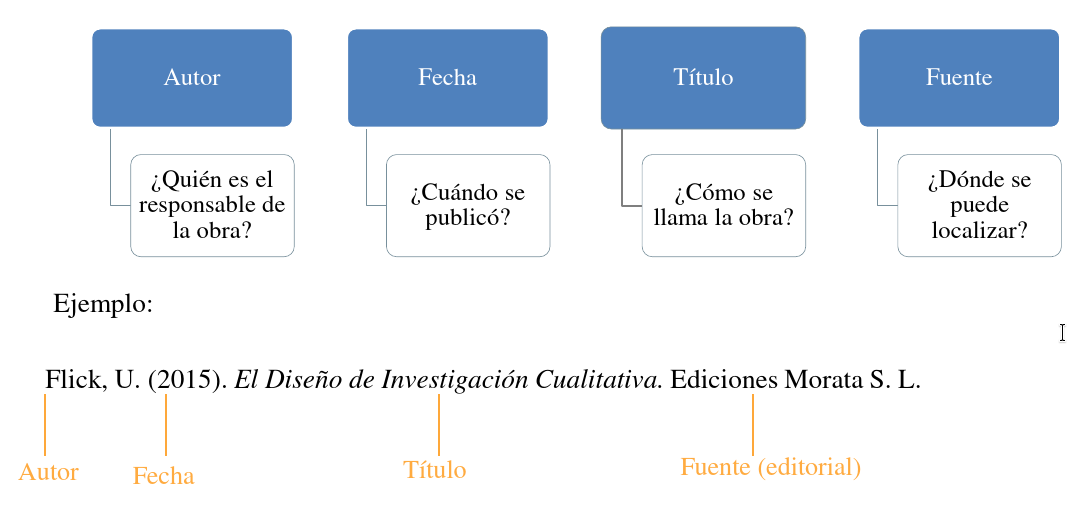
\includegraphics[width=1\linewidth]{images/screenshot008}
			\caption{parafraseo parentético}
			\label{fig:screenshot008}
		\end{figure}
	\end{exampleblock}

\end{frame}

\begin{frame}
	\frametitle{Libro}

	Cada libro trae en las primeras páginas una identificación que provee toda la
	información necesaria para realizar la referencia. Ejemplo:

	\begin{exampleblock}{}
\begin{figure}
	\centering
	
\includegraphics[width=0.4\linewidth]{images/screenshot009}
	\label{fig:screenshot009}
\end{figure}
	\end{exampleblock}

\end{frame}

\begin{frame}
	\frametitle{Forma básica para citar libros}

	Los libros son publicaciones extensas, que cuentan con el respaldo de una casa editorial y
	que están integrados por capítulos.

	\begin{exampleblock}{}
		\begin{figure}
			\centering
			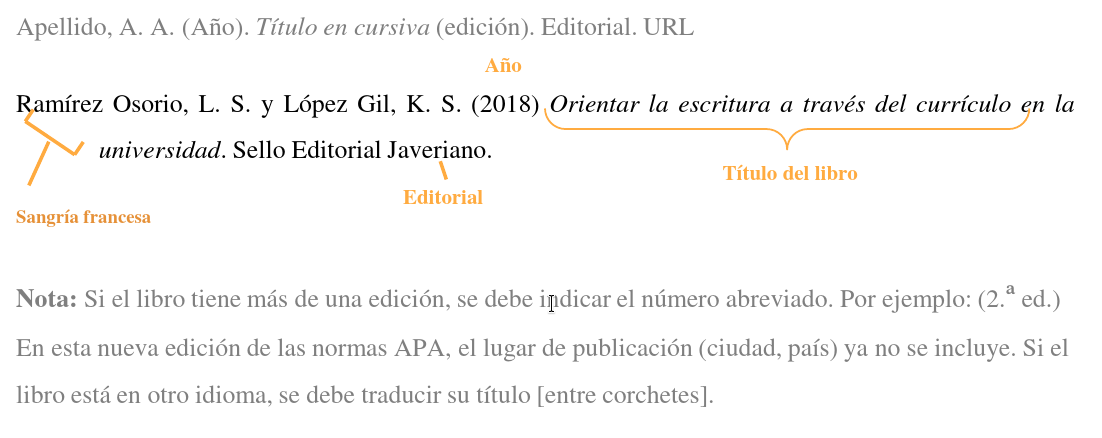
\includegraphics[width=1\linewidth]{images/screenshot010}
			\label{fig:screenshot010}
		\end{figure}
	\end{exampleblock}

\end{frame}

\begin{frame}
	\frametitle{Libro con autor}

	Libro en el que un autor o grupo de autores son los responsables de la obra completa.

	\begin{exampleblock}{}
		\begin{figure}
			\centering
			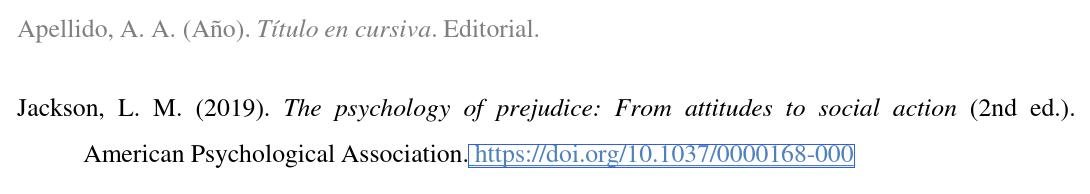
\includegraphics[width=1\linewidth]{images/screenshot011}
			\label{fig:screenshot010}
		\end{figure}
	\end{exampleblock}

\end{frame}

\begin{frame}
	\frametitle{Libro con editor}

	Libro que ha sido coordinado por un editor, pero que tiene distintos autores responsables de
	cada capítulo que integra la obra.

	\begin{exampleblock}{}
		\begin{figure}
			\centering
			
\includegraphics[width=1\linewidth]{images/screenshot012}
			\label{fig:screenshot010}
		\end{figure}
	\end{exampleblock}

\end{frame}

\begin{frame}
	\frametitle{Artículos científicos (Journal)}

	Los artículos científicos son publicaciones primarias que aparecen en revistas especializadas.
	Pueden aparecer en versión impresa, digital o ambas. La información para realizar la referencia de un
	artículo se suele encontrar en la primera página del artículo, en la parte superior o en el pie de página.

	\begin{exampleblock}{}
		\begin{figure}
			\centering
			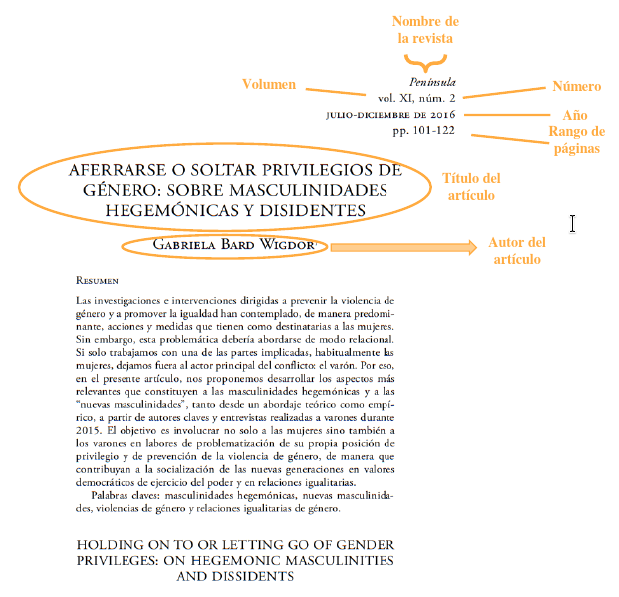
\includegraphics[width=0.5\linewidth]{images/screenshot013}
			\label{fig:screenshot010}
		\end{figure}
	\end{exampleblock}

\end{frame}

\begin{frame}
	\frametitle{Forma básica de los artículos científicos}

	\begin{exampleblock}{}
		\begin{figure}
			\centering
			
\includegraphics[width=1\linewidth]{images/screenshot014}
			\label{fig:screenshot010}
		\end{figure}
	\end{exampleblock}

	\textbf{Artículo impreso}

	\begin{exampleblock}{}
		\begin{figure}
			\centering
			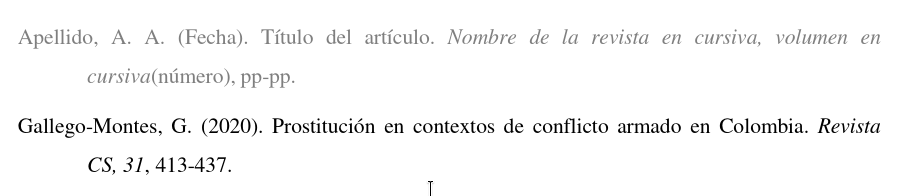
\includegraphics[width=1\linewidth]{images/screenshot015}
			\label{fig:screenshot010}
		\end{figure}
	\end{exampleblock}

\end{frame}

\begin{frame}
	\frametitle{Forma básica de los artículos científicos}

	\textbf{Artículo en línea}

	\begin{exampleblock}{}
		\begin{figure}
			\centering
			
\includegraphics[width=1\linewidth]{images/screenshot016}
			\label{fig:screenshot010}
		\end{figure}
	\end{exampleblock}

	\textbf{Artículo impreso}

	\begin{exampleblock}{}
		\begin{figure}
			\centering
			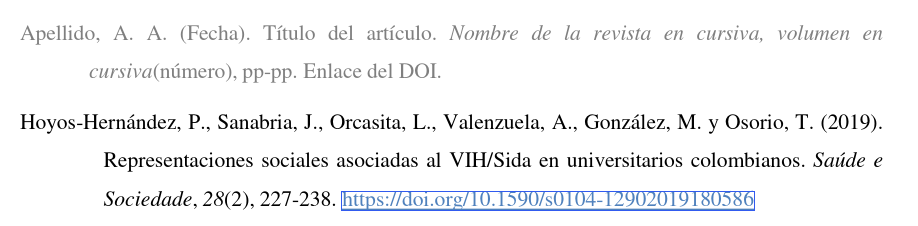
\includegraphics[width=1\linewidth]{images/screenshot017}
			\label{fig:screenshot010}
		\end{figure}
	\end{exampleblock}

\end{frame}



% Sección 8
\section{Técnicas de parafraseo}

% Sección 9
\section{Formato}

% Sección 10
\section{Estilo Vancouver}

% Sección 11
\section{Tablas, Figuras y Notas}

%----------------------------------------------------------------------------------------
%	CLOSING SLIDE
%----------------------------------------------------------------------------------------

\begin{frame}[plain] % The optional argument 'plain' hides the headline and footline
	\begin{center}
		{\Huge The End}

		\bigskip\bigskip % Vertical whitespace

		{\LARGE Questions? Comments?}
	\end{center}
\end{frame}

%----------------------------------------------------------------------------------------
\end{document}
